%%%%%%%%%%%%%%%%%%%%%%%%%%%%%%%%%%%%%%%%%%%%%%%%%%%%%%%%%%%%%%%%%%%%%%%%%%%%%%%%%%%%%%%%%%%%%%%%%%%
% Chapter 2 -> Background
% Author: Mingbo Cheng
%%%%%%%%%%%%%%%%%%%%%%%%%%%%%%%%%%%%%%%%%%%%%%%%%%%%%%%%%%%%%%%%%%%%%%%%%%%%%%%%%%%%%%%%%%%%%%%%%%%
\chapter{Background}
\label{cha:background}

\graphicspath{{chapter2/figs/}}

Background


\section{DNA Organization, chromatin accessibility and gene regulation}
In the symphony of life, the function of DNA organization, chromatin accessibility, and gene regulation orchestrates a harmonious dance that dictates the fate and functioning of every living organism. We start this section by first introducing DNA organization. Next, we talk about chromatin accessibility followed by the introduction of gene regulation.

\subsection{DNA Organization: The Architectural Blueprint of Life}
Deoxyribonucleic Acid, or DNA is the genetic blueprint of life, containing the instructions for the development and functioning of living organisms. It is a long, double-stranded helical structure composed of four nucleotide building blocks: adenine (A), thymine (T), cytosine (C), and guanine (G). The sequence of these nucleotides forms the genetic code, encoding instructions for the development, functioning, and maintenance of all living organisms. DNA is organized into structures called chromosomes, which are located in the cell nucleus.

\subsection{Chromatin accessibility: Gatekeepers of the Genetic Code}
Chromatin is the complex of DNA and proteins found in the nucleus of a cell. Chromatin accessibility is a crucial molecular concept that describes the degree to which DNA is available or accessible for cellular processes, particularly gene expression. It can exist in two states: open and condensed. Open chromatin refers to the relaxed, accessible state where DNA is available for transcription and gene expression. In this state, the DNA is not tightly wound around histone proteins, allowing regulatory proteins and RNA polymerase to easily access specific DNA sequences, facilitating the transcription of genes into RNA. Open chromatin is associated with active gene expression and is influenced by various factors, including epigenetic modifications such as acetylation and methylation. Conversely, in a "closed" or condensed chromatin state, the DNA is tightly wound around histone proteins, making it less accessible. This state inhibits the binding of transcriptional machinery, leading to reduced or suppressed gene expression. Closed chromatin is associated with inactive or silenced genes.

\subsection{Gene Regulation: The Symphony's Conductor}
Gene regulation refers to the mechanisms that control the expression of genes. While an organism's DNA carries the instructions for a vast array of biological processes, not all genes are active all the time. Gene regulation allows cells to turn genes on or off, and to fine-tune their activity. This regulation is achieved through the interaction of regulatory proteins, transcription factors, and other molecules that bind to specific DNA sequences, influencing the initiation or inhibition of transcription. Epigenetic modifications, such as DNA methylation and histone modification, also play a crucial role in gene regulation by modifying the accessibility of DNA.


\begin{figure}[!ht]
	\centering
	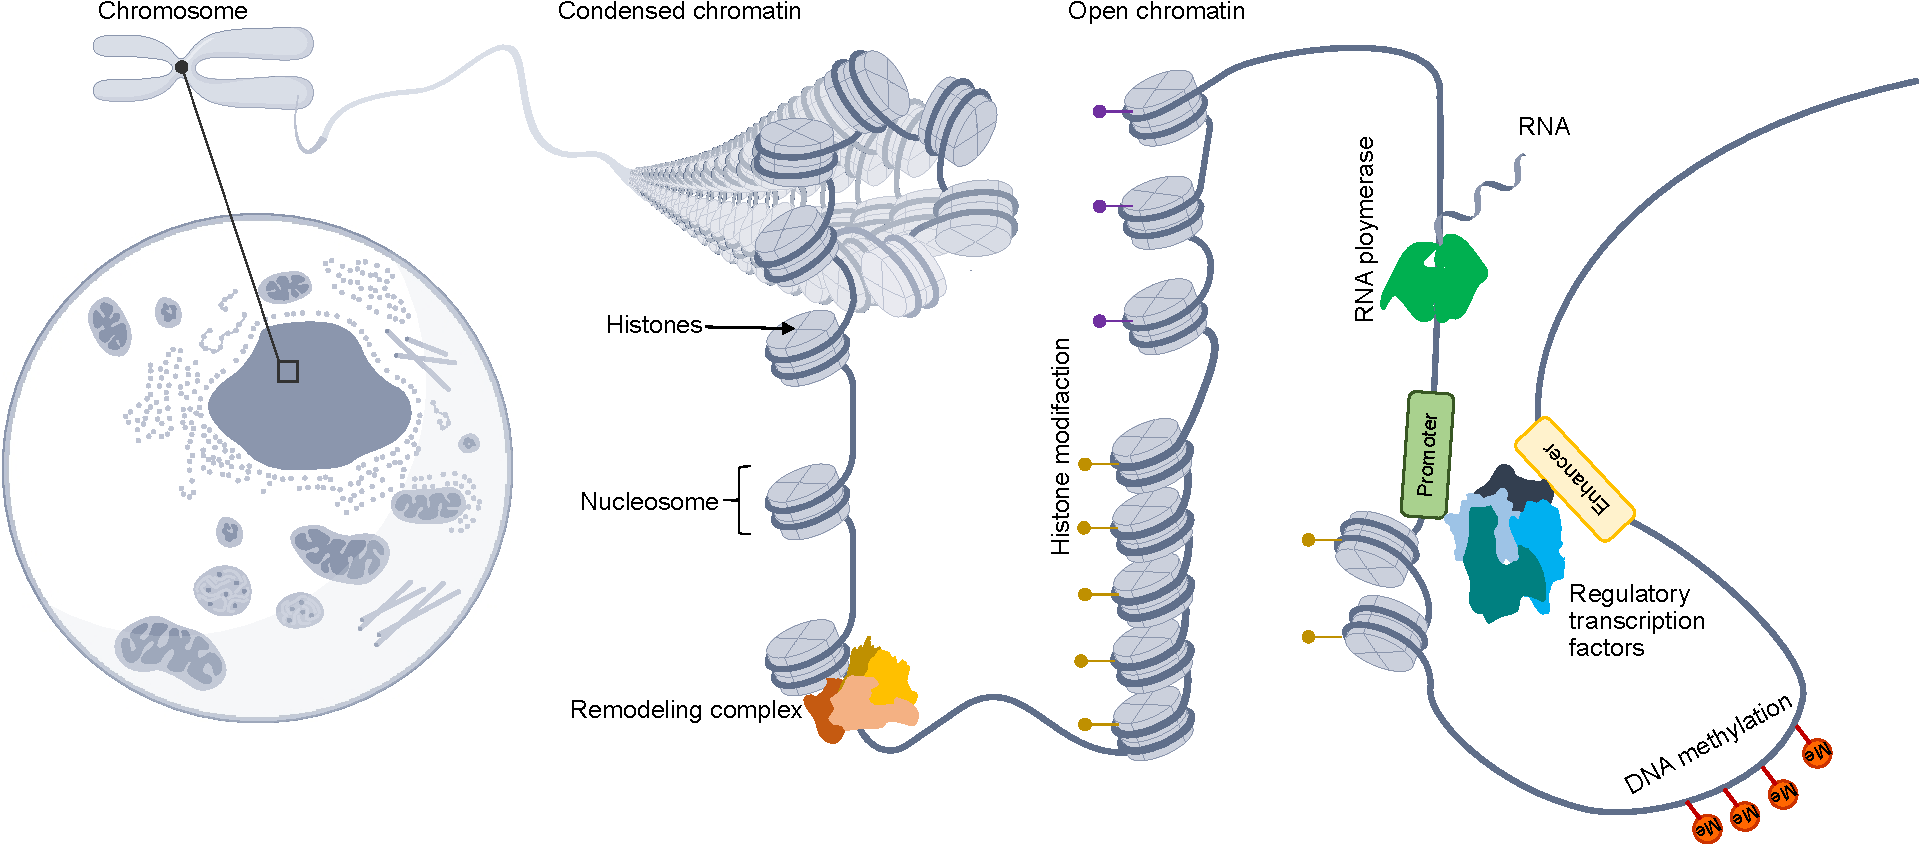
\includegraphics[width=0.95\textwidth]{chromatin_organization/fig}
	\vspace{0.1cm}
	\caption[chromatin\_organization.]{
	chromatin\_organization.}
	\label{fig:chromatin_organization}
\end{figure}



\section{Single cell sequencing technology}
Since Sanger sequencing~\cite{sanger1975rapid} analysis was introduced in 1975, numerous advances in methodology have been developed to improve the understanding of the heterogeneity and transcriptomic states present in complex biological systems. The invention of a series of rapidly evolving Next Generation Sequencing (NGS) technologies revolutionarily facilitates the study of heterogeneous biological processes with high throughput, shorter time and lower cost. NGS enables researchers to perform profiling of epigenome, transcriptiomes and proteomoes. The development of single cell sequencing technology further enables the study of heterogeneity at single cell resolution. In this section, we will briefly introduce the single cell sequencing technology,  single cell RNA sequencing, single cell ATAC sequencing and single cell protein sequencing.


\begin{figure}[!ht]
	\centering
	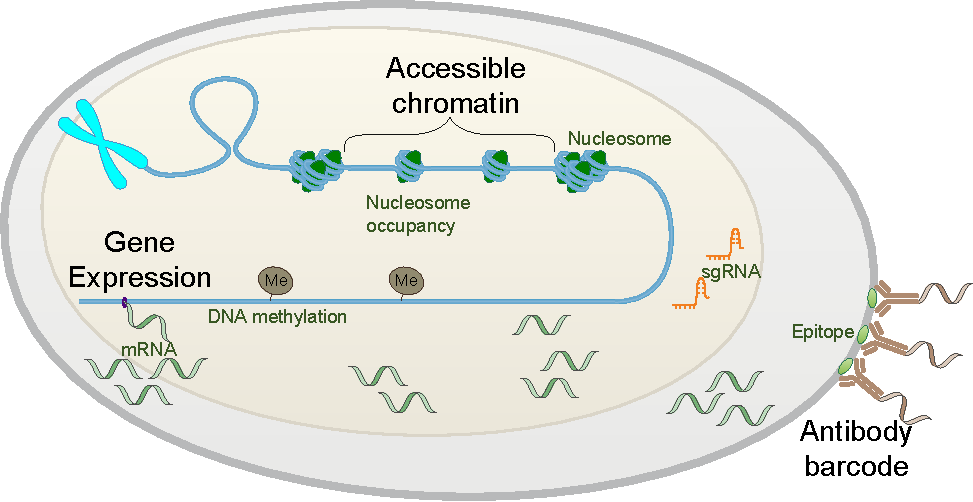
\includegraphics[width=0.95\textwidth]{multimodal-single-cell/fig}
	\vspace{0.1cm}
	\caption[mulitmodal single celll.]{multimodal singel cell. \emph{Source: ~\cite{zhu2020single}}(modified to fit thesis format and/or clarify key points)}
	\label{fig:multimodal_single_cell}
\end{figure}



\subsection{Transcriptomics profiling with scRNA-seq}

\begin{figure}[!ht]
	\centering
	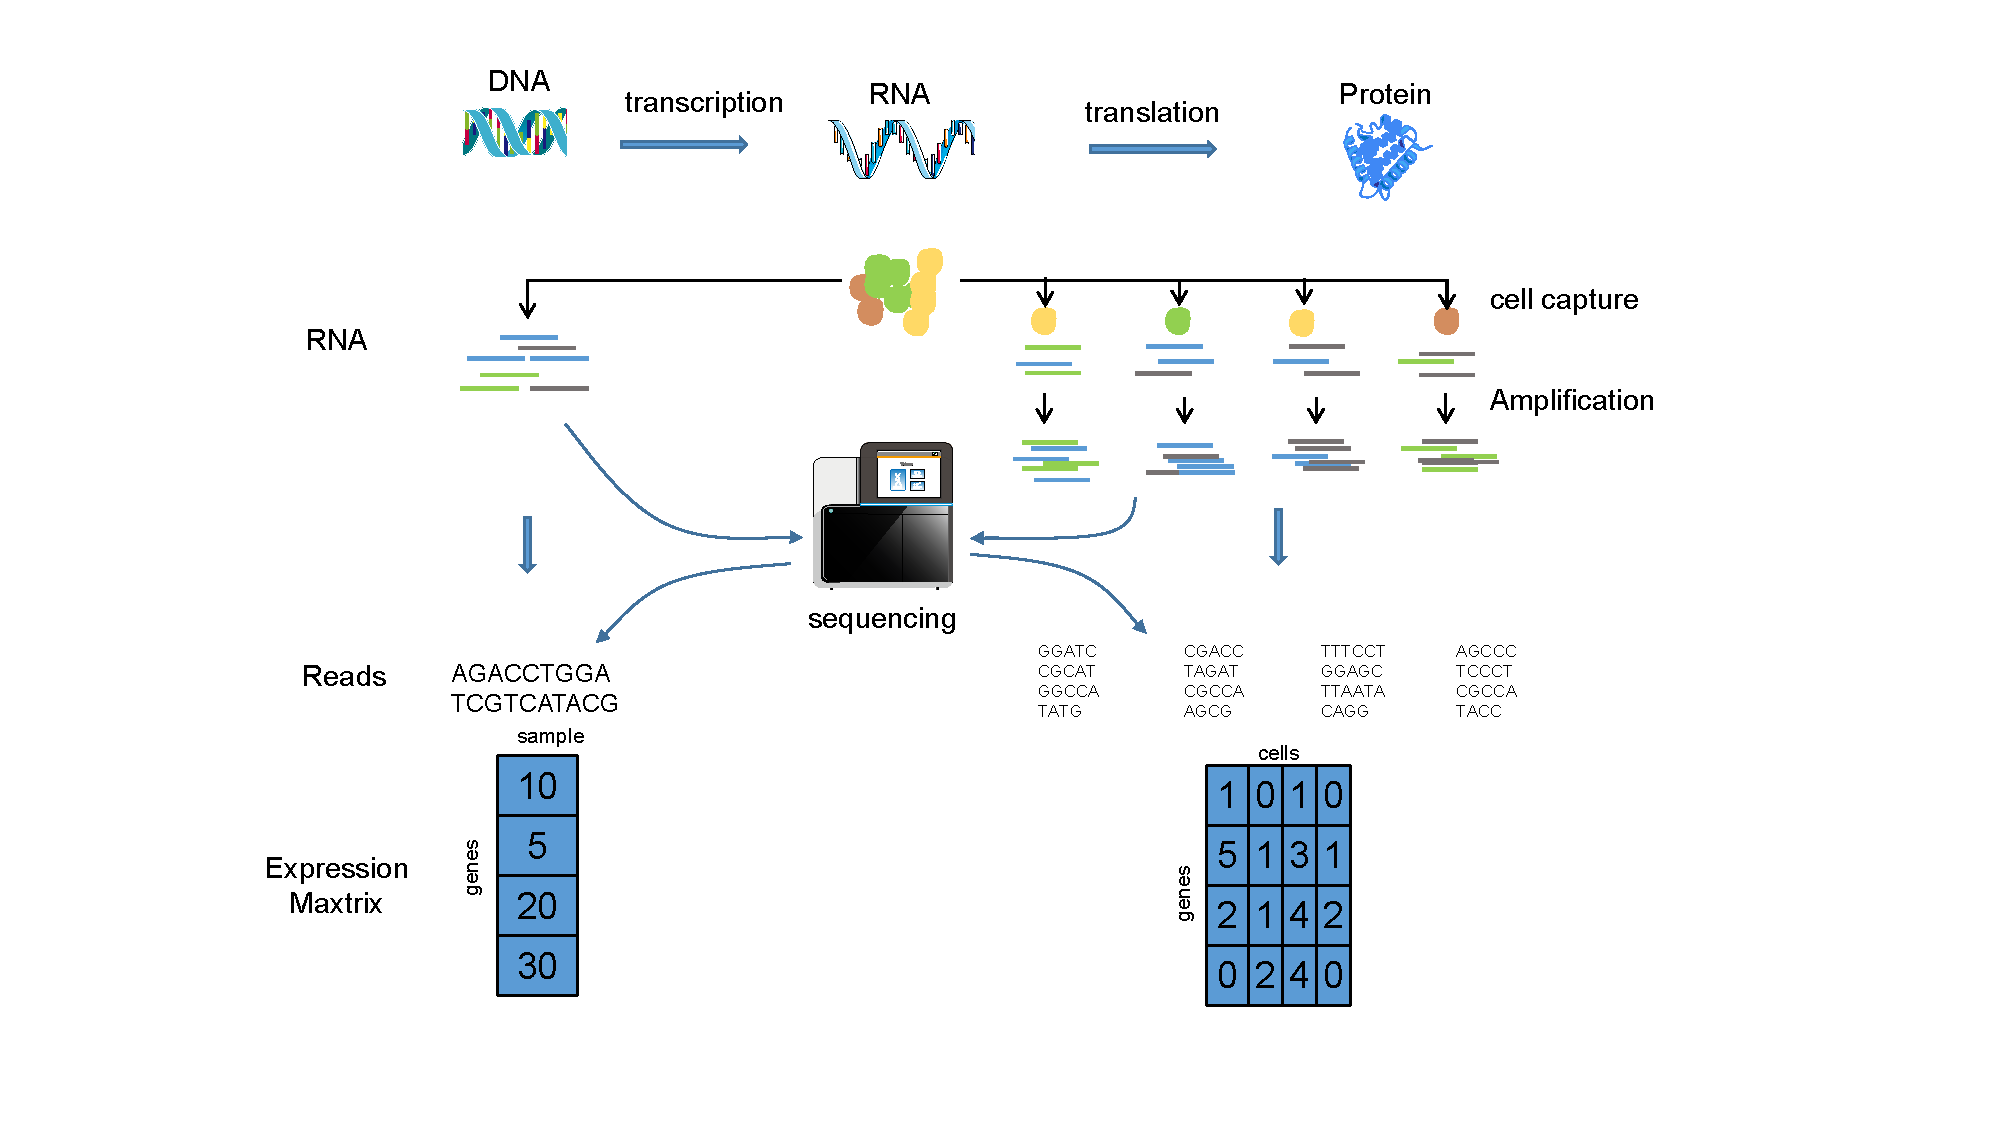
\includegraphics[width=0.95\textwidth]{rna_scRNA/fig}
	\vspace{0.1cm}
	\caption[bulk rna and single cell rna sequencing.]{bulk rna and single cell rna sequencing.}
	\label{fig:rna_scRNA}
\end{figure}


Single cell RNA sequencing(scRNA-seq)~\cite{singlecellsequencing2014, singlecellsequencing2015} was introduced in 2009~\cite{tang2009mrna}. In general, scRNA-seq protocols can be classified into droplet-based and plate-based methods. Droplet-based methods use droplet microfluidics technology~\cite{dropletcompare2019, droplet2019practice} to capture cells in each droplets. Drop-seq~\cite{dropseq2015} inDrop~\cite{indrop2015} and GemCode/Chromium 10X~\cite{zheng2017massively} use microfluidic droplet chemistry with encapsulation of cells and barcoding beads~\cite{rotem2015high}. Plate-based methods use microwell plates to capture cells in each well. SMART-seq~\cite{smartseq2012} and SMART-seq2~\cite{smartseq22014} use microwell plates to capture cells in each well. The microwell plates are pre-coated with oligo-dT primers. The captured cells are lysed and the RNA is reverse transcribed into cDNA. The cDNA is then amplified by PCR. The amplified cDNA is then sequenced by NGS. The plate-based methods are more expensive and time-consuming, but they have higher sensitivity and lower dropout rate. The droplet-based methods are cheaper and faster, but they have higher dropout rate and lower sensitivity. The droplet-based methods are more suitable for large scale studies, while the plate-based methods are more suitable for small scale studies.

%


\subsection{Chromatin accessibility profiling with scATAC-seq}
Chromatin accessibility profiling using Single-Cell Assay for Transposase-Accessible Chromatin sequencing, or scATAC-seq, has emerged as a revolutionary tool, allowing scientists to unravel the dynamic landscape of chromatin accessibility at a single-cell resolution. This technology not only provides a detailed map of regulatory elements within individual cells but also promises to deepen our understanding of cellular heterogeneity, development, and the intricate orchestration of gene regulation in health and disease. Join us as we delve into the profound insights that chromatin accessibility profiling with scATAC-seq brings to the forefront of genomic research, unlocking the secrets of cellular diversity at an unprecedented level of granularity. ATAC-seq use xxxx, see  

%\subsection{Protein profiling in single cell}
%Protein analysis at the single cell level has relied on the use of antibodies that bind specifically to target proteins. Flow cytometry uses fluorescently labeled antibodies to convert protein signals into fluorescence signals~\cite{@article{kim2022single}

\begin{figure}[!ht]
	\centering
	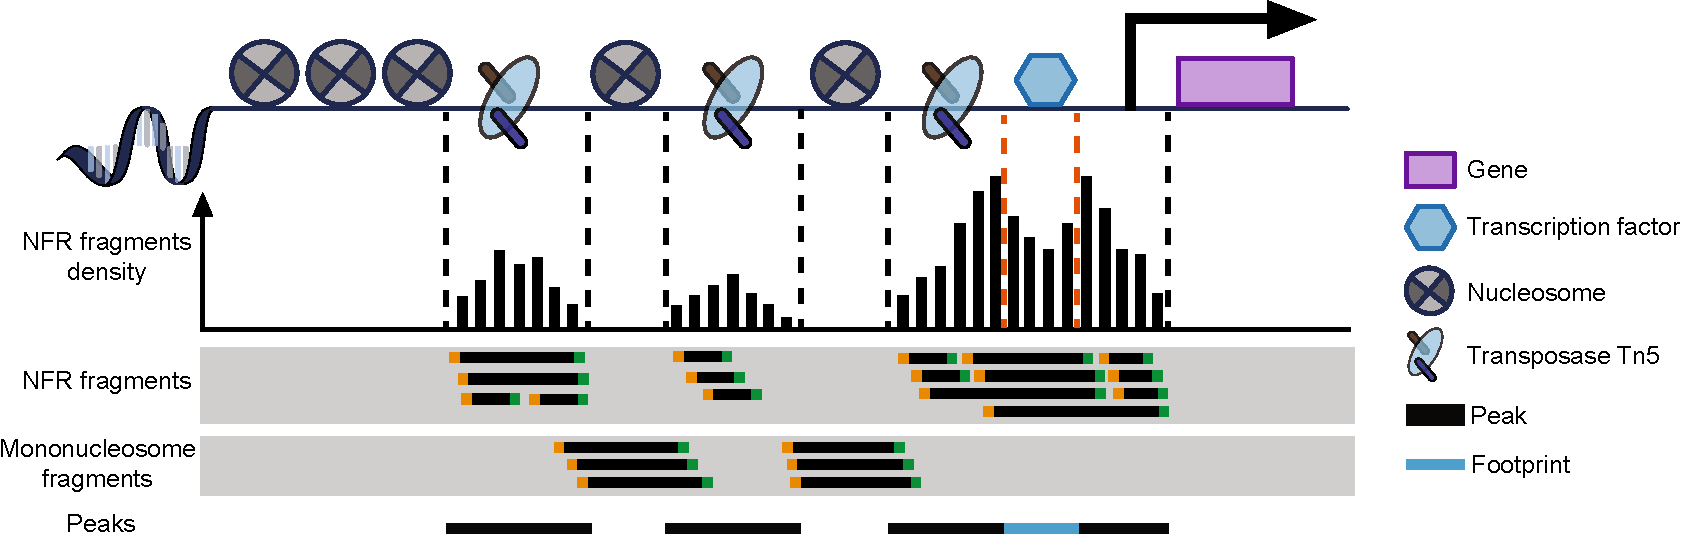
\includegraphics[width=0.95\textwidth]{ATAC-seq/fig}
	\vspace{0.1cm}
	\caption[ATAC sequenceing.]{ATAC sequencing. \emph{Source: ~\cite{yan2020reads}} (modified to fit thesis format and/or clarify key points)}
	\label{fig:ATAC-seq}
\end{figure}


\subsection{Simultaneous multi-modal profiling of single cell}
Single-cell multi-modal technologies typically analyze various types of molecules within a single cell, providing a more profound understanding of biology compared to studying individual molecular layers from separate cells. These advanced technologies unveil cellular heterogeneity across multiple molecular levels within a cell population, offering insights into the interconnectedness or independence of variation across different modalities. The datasets produced by these techniques hold the potential to facilitate a more comprehensive comprehension of the fundamental biological processes and mechanisms that contribute to cellular heterogeneity. Furthermore, they shed light on the associations between normal development, aging, disease etiology, and the intricate links between these phenomena. A variety of multi-modal profiling methods have been proposed recently, see figure Table.\ref{tab:multimodal-methods}

\begin{table}[!ht]
	\footnotesize
	\centering
	\begin{tabular}{lll}%{0.1\linewidth}}
		\toprule
		{\textbf{Modalities}}  & {\textbf{Protocols}} & {\textbf{reference}} \\ 
		\midrule
		\multirow{5}{*}{\shortstack[l]{
\includegraphics[scale=1]{multi-model-methods/Protein_RNA.pdf}}}
		   & PLAYR & {~\cite{frei2016playr}} \\
		   & CITE-seq & {~\cite{stoeckius2017citeseq}} \\
           & REAP-seq & {~\cite{peterson2017reapseq}}\\
           & RAID & {~\cite{Gerlach2019RAID}} \\
		   & ECCITE-seq &  {\cite{mimitou2019ECCITE}}\\
		\midrule
		\multirow{5}{*}{\shortstack[l]{
\includegraphics[scale=1]{multi-model-methods/RNA_ATAC.pdf}}}
		   & sci-CAR & {~\cite{cao2018scicar}}\\
           & SNARE-seq & {~\cite{chen2019SNARE}} \\
           & scNMT-seq & {~\cite{clark2018scnmt}}\\
		   & scCAT-seq &  {~\cite{liu2019scCAT}} \\ 
           & multiome & 10x Genomics\\
		\midrule
		\multirow{5}{*}{\shortstack[l]{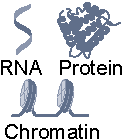
\includegraphics[scale=1]{multi-model-methods/3.pdf}}}
		& TEA-seq & {~\cite{swanson2021simultaneous}}\\
		& DOGMA-seq & ~\cite{mimitou2021scalable} \\
		\\
		\\
		\\
		\bottomrule
	\end{tabular}
	\vspace{0.1cm}
	\caption[Major multimodal methods]{major multimodal methods.}
	\label{tab:multimodal-methods}
\end{table}






\begin{figure}[!ht]
	\centering
	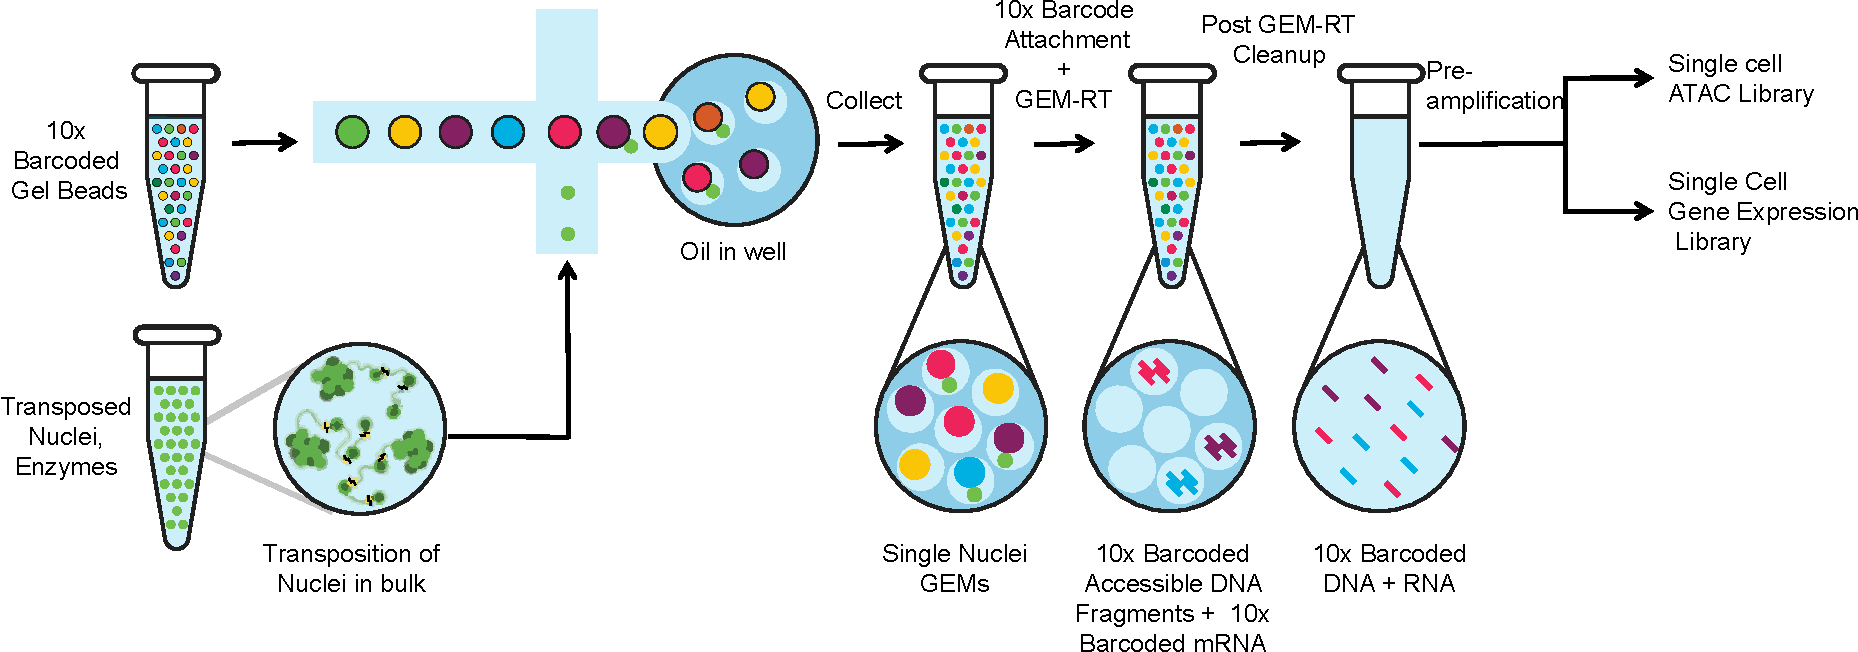
\includegraphics[width=0.95\textwidth]{droplets_multiome_scRNA_scATAC/fig}
	\vspace{0.1cm}
	\caption[droplets\_multiome\_scRNA\_scATAC.]{droplets\_multiome\_scRNA\_scATAC. \emph{Source: ~\cite{satpathy2019massively}} (modified to fit thesis format and/or clarify key points)}
	\label{fig:droplets_multiome_scRNA_scATAC}
\end{figure}

\section{Computational analysis of single cell}
\begin{figure}[!ht]
	\centering
	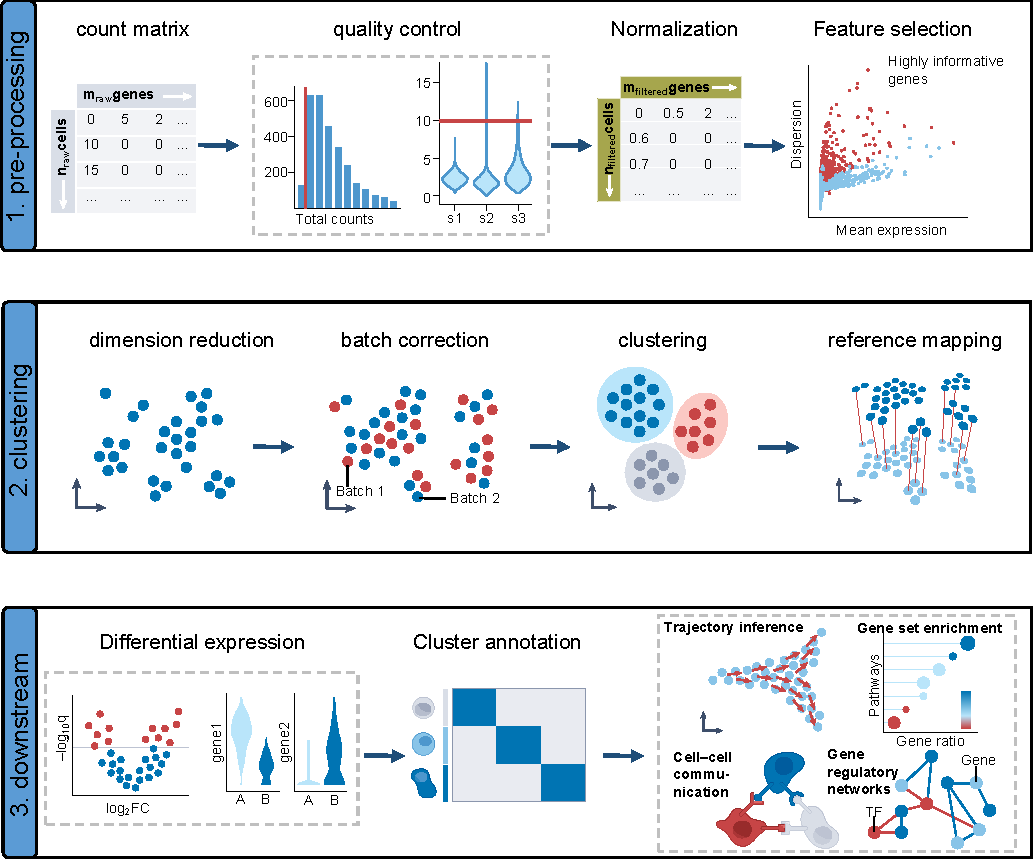
\includegraphics[width=0.95\textwidth]{workflow_scRNA/fig}
	\vspace{0.1cm}
	\caption[workflow\_scRNA.]{workflow scRNA. \emph{Source: ~\cite{heumos2023best}} (modified to fit thesis format and/or clarify key points)}
	\label{fig:workflow_scRNA}
\end{figure}

\begin{figure}[!ht]
	\centering
	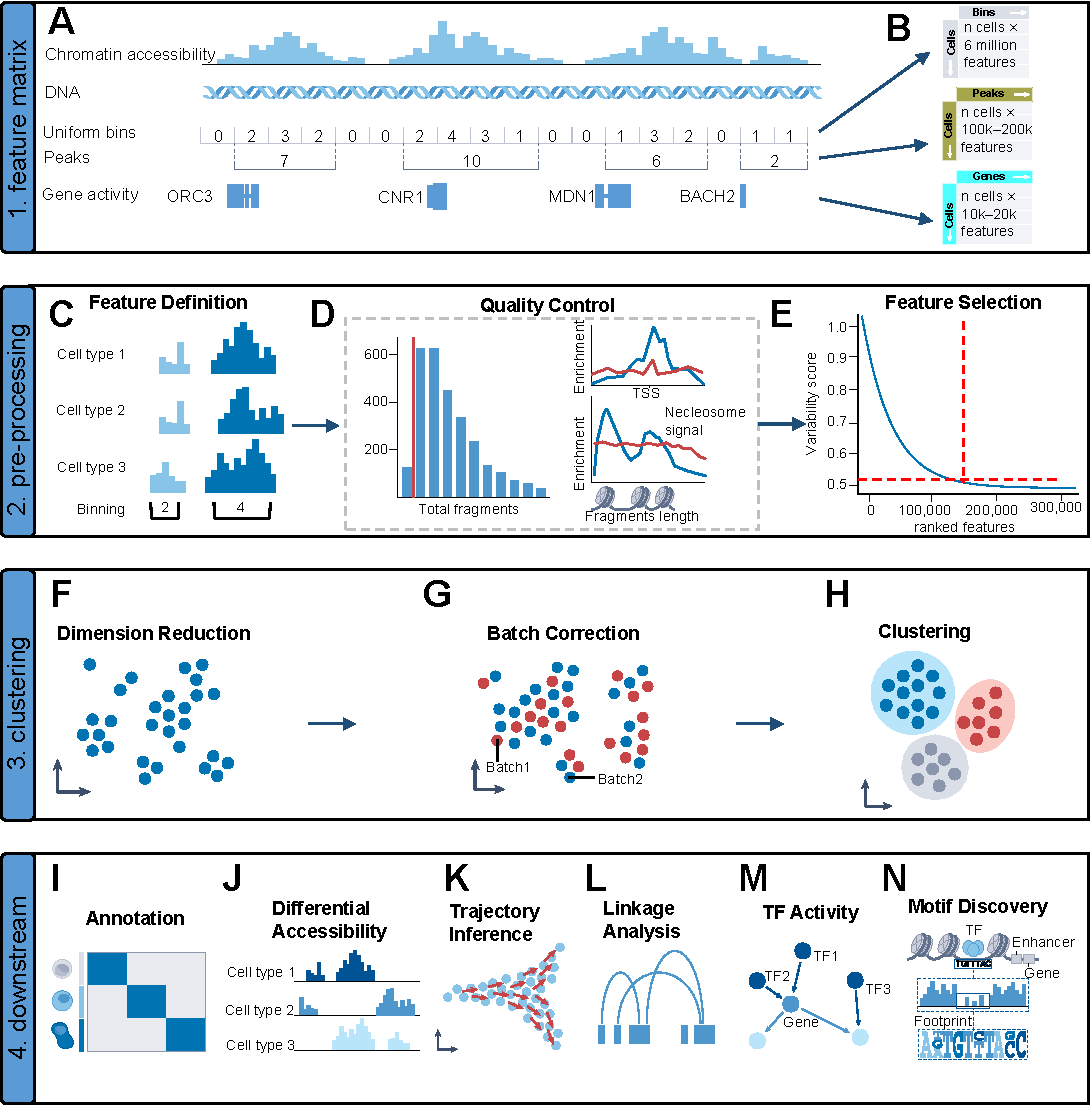
\includegraphics[width=0.95\textwidth]{workflow_scATAC/fig}
	\vspace{0.1cm}
	\caption[workflow\_scATAC.]{workflow scATAC  \emph{Source: ~\cite{heumos2023best}} (modified to fit thesis format and/or clarify key points)}
	\label{fig:workflow_scATAC}
\end{figure}

\begin{figure}[!ht]
	\centering
	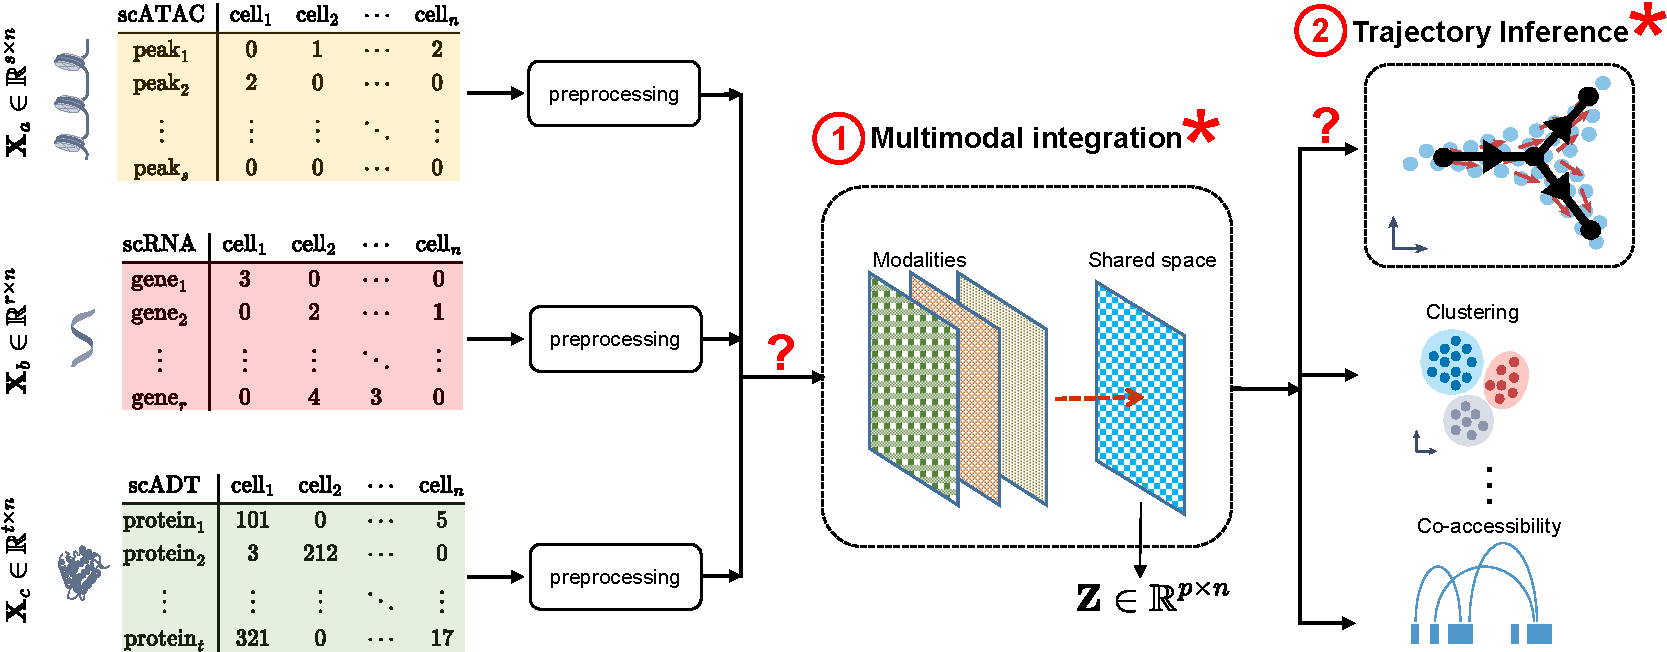
\includegraphics[width=0.95\textwidth]{workflow_multimodal/fig}
	\vspace{0.1cm}
	\caption[workflow\_multimodal.]{workflow\_multimodal}
	\label{fig:workflow_multimodal}
\end{figure}


\subsection{scRNA}
\subsubsection{pre-processing}
\subsubsection{Dimensional reduction and Clustering}
\subsubsection{Downstream analysis}

\subsection{scATAC}
\subsubsection{pre-processing}
\subsubsection{Dimensional reduction and Clustering}
\subsubsection{Downstream analysis}

%%might ignore the surface protein part
\subsection{surface protein}
\subsubsection{pre-processing}
\subsubsection{Dimensional reduction and Clustering}
\subsubsection{Downstream analysis}


\subsection{multi-modal analysis}


\subsubsection{preprocessing}
\subsubsection{Dimensional reduction, integration and clustering}
\subsubsection{Downstream analysis}


\section{Related works}
\subsection{Challenge of mulit-modal analysis}
% a figure shows the features types differences among different modalities

\begin{figure}[!ht]
	\centering
	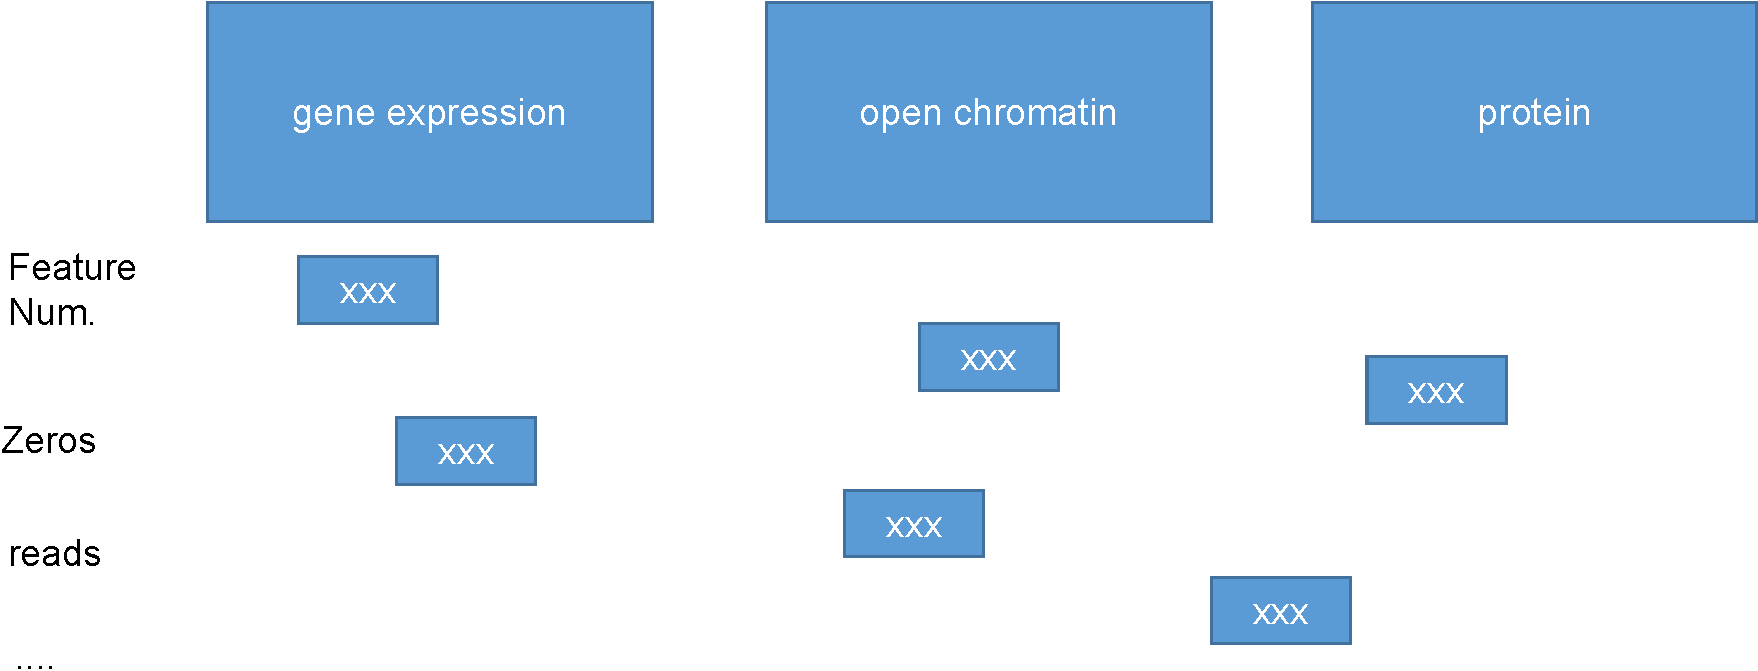
\includegraphics[width=0.95\textwidth]{modalities_differences/fig}
	\vspace{0.1cm}
	\caption[modalities\_differences.]{
	modalities\_differences.}
	\label{fig:modalities_differences}
\end{figure}



\subsection{Computational Methods for single cell multimodal integration}

\begin{figure}[!ht]
	\centering
	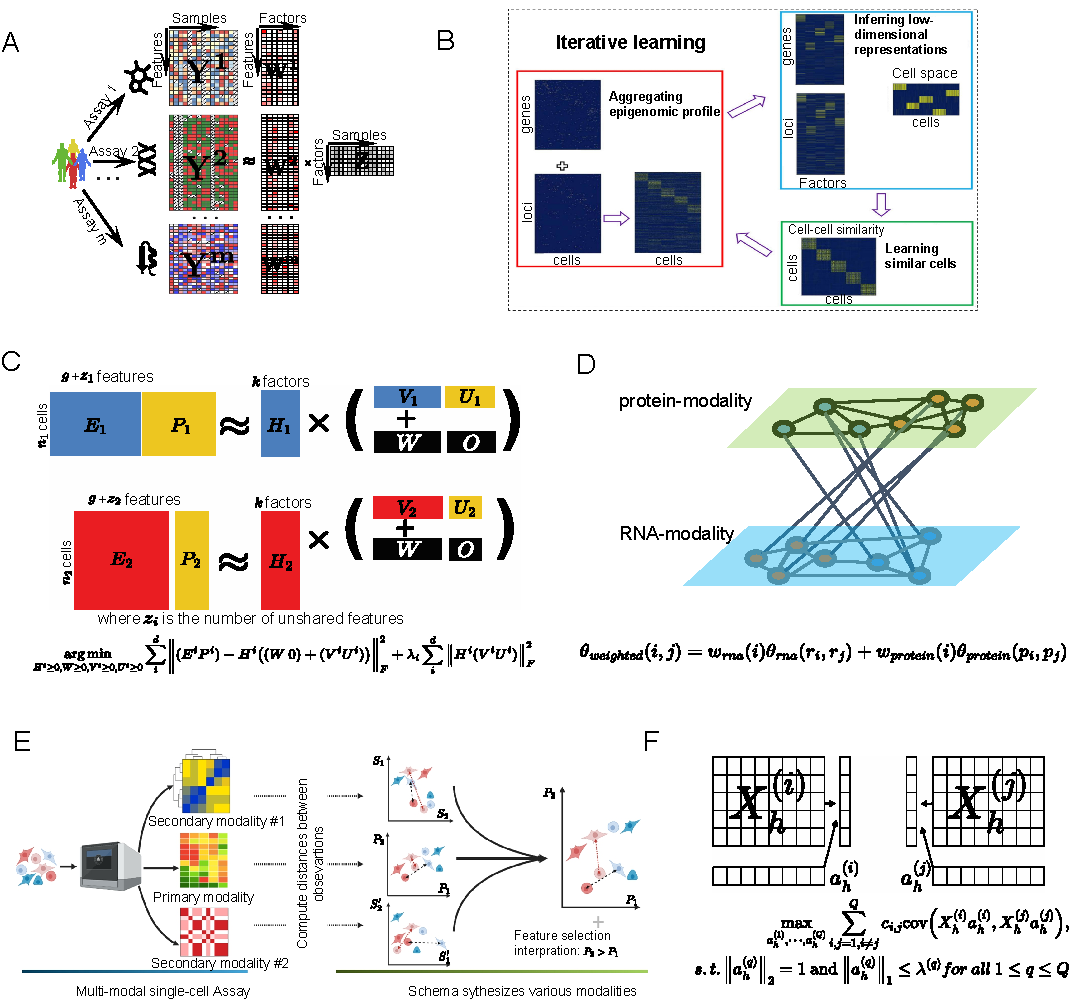
\includegraphics[width=0.95\textwidth]{multimodal_integration_methods_schematic/fig}
	\vspace{0.1cm}
	\caption[multimodal\_integration\_methods\_schematic.]{
	A) MOFA schematic B) scAI schematic C) Liger D) Seurat weighted nearest neighbor(WNN) E) schema  F) DIABLO . \emph{Source ~\cite{tewari2017mofa,jin2020scai,kriebel2022uinmf,hao2021integrated,singh2021schema,singh2019diablo}}(modified to fit thesis format and/or clarify key points)}
	\label{fig:multimodal_integration_methods_schematic}
\end{figure}



% table of single cell multimodal integration methods
\subsubsection{Schema}
Schema~\cite{singh2021schema}  applied metrics learning to reweigh modality features by maximizing the agreement with other modalities. Specifically, it utilizes quadratic programming (QP) to learn a scaling transformation $u$ for the primary matrix $X$ such that pairwise distances of the transformation $u *  x_i$ (where $*$ is coordinate-wise multiplication, for each $x_i\in X$) are highly correlated other modalities. Specifically, it assumes $N$ observations across $r$ datasets $D_j$, where $j=1,\cdots,r$ and $D_j  = \{x_i^{j}: i = 1,2,\cdots,N\}$ contains data for each observation. First, it refers $D_1$ as the primary modality and $D_2,\cdots,D_r$ as the secondary modalities. Next, it computes the pairwise distances $\rho_1,\cdots,\rho_j$ for each modality $D_j$ where $\rho_j(x_n^{j}, x_m^{(j)})$ is the distance between observation $n$ and $m$ in $D_j$. Then, it aims to find a transformation $\Omega$ with $\Omega(D)$ generating a dataset $D^{*}$ such that the Euclidean metric $\rho^{*}$ on $D^{*}$ on $D^{*}$ aligns the various metrics. $\Omega$ is limited to be a scaling transformation:
\begin{equation}
\Omega(D) = \{diag(u)x: x \in D\}
\end{equation}
where $u \in \mathbb{R}^{k}$ and  $diag(u)$ is a  $k\times k$ diagonal matrix with diagonal entries $u$. Then, the squared distance between points under the transformation is given by:
\begin{equation}
\rho^{*}(x_n, x_m) = \|diag(u)x_n - diag(u)x_m\|^2 = \|diag(w)(x_n - x_m)\|^2 
\end{equation}
where $w$ is the element-wise square of u. The scaling transforms u acts as a feature-weighting mechanism to choose the features of $D_1$ that align the datasets best. Schema integrates between the metrics $\rho_j$ to learn a metric $\rho^{*}$ that aligns well with all of them. The correlation between $\rho^{*}$ and $\rho_j$ is measured by the Pearson correlation coefficient:
\begin{equation}
	\text{corr}(\rho^{*}, \rho_j) = \frac{\text{cov}(\rho^{*}, \rho_j)}{\text{var}(\rho^{*})\text{var}(\rho_j)}
\end{equation}
To tackle multiple modalities, Schema maximizes the sum of Pearson correlation between $\rho^{*}$ and all other modalities pairwise distances $\rho_2,\cdots,\rho_j$:
\begin{equation}
	\left\{\sum_{j=2}^r \gamma_j \text{corr}(\rho^{*}(w), \rho_j)\right\} \text{ subject to corr}(\rho^{*}(w), \rho_1) \geq s 
\end{equation}
Where $\gamma_j$ and s are hyperparameters that determine the importance of the various metrics.


\subsubsection{Seurat WNN}
Weighted nearest neighbor (WNN)~\cite{hao2021integrated} constructs a single unified representation across multiple modalities. It takes CITE-seq~\cite{citeseq2017} with scRNA and protein modalities for example to explain the algorithm. First, it creates k-nearest neighbor graphs for each modality based on the pre-computed latent representation of each feature matrix. Where $r_i$ represents the L2-normalized latent representation of $cell_i$ in modality RNA and $p_i$ represents the L2-normalized latent representation of $cell_i$ in modality protein. $\{knn_{r,i,1}\cdots knn_{r,i,k}\}$ is the set of $k$-nearest RNA neighbors of cell $i$ and $\{knn_{p,i,1}\cdots knn_{p,i,k}\}$ is the set of $k$-nearest protein neighbors of cell $i$. Next, it predicts cell $i$ modality profile within and across modalities, the within modality prediction is:
\begin{equation}
	\begin{aligned}
		&\hat{r}_{i, knn_r}=\frac{\sum_{j=1}^{k} r_{k n n_{r, i, j}}}{k} \\
		&\hat{p}_{i, knn_p}=\frac{\sum_{j=1}^{k} p_{k n n_{p, i, j}}}{k} 
	\end{aligned}
\end{equation}

The across modalities prediction is:
\begin{equation}
	\begin{aligned}
		&\hat{r}_{i, knn_p}=\frac{\sum_{j=1}^{k} r_{k n n_{p, i, j}}}{k} \\
		&\hat{p}_{i, knn_r}=\frac{\sum_{j=1}^{k} p_{k n n_{r, i, j}}}{k}
	\end{aligned}
\end{equation}

Next, it calculates affinities using the exponential kernel utilized in UMAP(McInnes et al., 2018) between each cell $i$ and its KNN(of each modality) average profile, specifically, the affinities between $cell_i$ and its KNN average profile within modality RNA and modality protein are:
\begin{equation}
	\begin{aligned}
		& \theta_{rna}\left(r_i,\hat{r}_{i, knn_r}\right) = \exp\left( \frac{-\max(d(r_i, \hat{r}_{i,knn_r}))-d(r_i, r_{knn_{r,i,1}}), 0)}{\sigma_{r,i} - d(r_i,r_{knn_{r,i,1}})}\right)\\
		& \theta_{protein}\left(p_i,\hat{p}_{i, knn_p}\right) = \exp\left( \frac{-\max(d(p_i, \hat{p}_{i,knn_p}))-d(p_i, p_{knn_{p,i,1}}), 0)}{\sigma_{p,i} - d(p_i,p_{knn_{p,i,1}})}\right)\\
	\end{aligned}
\end{equation}
Where $d(\cdot,\cdot)$ is the Euclidean distance, $\sigma_{r, i}$ and $\sigma_{p, i}$ is the bandwidth of RNA and protein kernels of cell $i$. The affinities between $cell_i$ and its KNN average profile across modalities are:
\begin{equation}
	\begin{aligned}
		& \theta_{rna}\left(r_i, \hat{r}_{i,knn_p}\right) = \exp\left( \frac{-\max(d(r_i, \hat{r}_{i,knn_p}))-d(r_i, r_{knn_{p,i,1}}), 0)}{\sigma_{p,i} - d(r_i,r_{knn_{p,i,1}})}\right)\\
		& \theta_{protein}\left(p_i, \hat{p}_{i,knn_r}\right) = \exp\left( \frac{-\max(d(p_i, \hat{p}_{i,knn_r}))-d(p_i, p_{knn_{r,i,1}}), 0)}{\sigma_{r,i} - d(p_i,p_{knn_{r,j,1}})}\right)\\
	\end{aligned}
\end{equation}
Next, for each modality, it applies softmax transformation to the pairwise ratio of affinity based on its own KNN and the counterpart affinity on other modalities as $\textbf{w}_rna(i)$ and $\textbf{w}_protein(i)$:
\begin{equation}
	\begin{aligned}
	& \textbf{w}_{rna}(i)=\frac{e^{(S_{rna}(i))}}{e^{S_{rna}(i)} + e^{S_{protein}(i)}}\\
	& \textbf{w}_{protein}(i)=\frac{e^{(S_{protein}(i))}}{e^{S_{rna}(i)} + e^{S_{protein}(i)}}
	\end{aligned}
\end{equation}
Where $S_{rna}(i) = \theta_{rna}(r_i, \hat{r}_{i,knn_r})/(\theta_{rna}(r_i, \hat{r_{i,knn_p}}) + \epsilon)$, and $S_{protein}(i) = \theta_{protein}(p_i, \hat{p}_{i,knn_p})/(\theta_{protein}(p_i, \hat{p_{i,knn_r}}) + \epsilon)$, the $\epsilon(10^{-4})$ is the small value to avoid zero division.

Finally, it calculates the weighted similarity between $cell_i$ and $cell_j$ as the dot product of $\textbf{w}_{rna}(i)$ and $\textbf{w}_{protein}(i)$:
\begin{equation}
	\theta_{weighted}(i,j)=\textbf{w}_{rna}(i)\theta_{rna}(r_i,r_j) + \textbf{w}_{protein}(i)\theta_{protein}(p_i,pj)
\end{equation}
It next constructs a WNN graph, as a KNN graph constructed using the weighted similarity metric. When there are more than two modalities($m$), similarly, it calculated the weighted similarity between $cell_i$ and $cell_j$ as the dot product of $\textbf{w}_m(i)$ and $\theta(i,j)$,
\begin{equation}
	\theta_{weighted}(i,j)=\sum_{m} \textbf{w}_m(i)\theta(i,j)
\end{equation}
Where $\theta(i,j)$ denotes the affinity between cell $i$ and cell $j$ in modality $m$.

\subsubsection{scAI}
scAI ~\cite{jin2020scai} is aimed to integrate multiple modalities with different feature types specific for scRNA $(X_1\in \mathbb{R}^{p \textbf{ genes} \times n \textbf{ cells}})$ and scATAC/DNA methylation$(X_2\in \mathbb{R}^{q \textbf{ loci}\times n \textbf{ cells}})$ modalities. It creates a matrix factorization model:
\begin{equation}
\min_{w_1,W_2,H,Z\geq 0} \alpha \|X_1-W_1H\|_F^2 + \|X_2(Z \circ R)-W_2H\|_F^2 + \lambda \|Z-H^\top H\|_F^2 + \gamma\sum_j \|H_{.j}\|_1^2
\end{equation}
Where $W_1$ and $W_2$ are the gene loading and locus loading matrices with size $p\times K$ and $q\times K$($K$ is rank), respectively. Each of the $K$ columns is considered as a factor to capture a biological process/signal relating to a specific cell type. $W_1^{ik}$ and $W_2^{ik}$ are the loading values of gene $i$ and locus $i$ in factor $k$, and the loading values represent the contributions of gene $i$ and locus $i$ in factor k. $H$ is the cell loading matrix with size $K\times n$($H_{.j}$ is the $j$th column of $H$), and the entry $H^{kj}$ is the loading value of cell $j$ when mapped onto factor $k$. $Z$ is the cell-cell similarity matrix. $R$ is a binary matrix generated by a binomial distribution with a probability $s$. $\alpha, \lambda, \gamma$ are regularization parameters, and the symbol $\circ$ represents dot multiplication.
The optimization problem is solved by a multiplicative update algorithm. The algorithm iteratively updates $W_1, W_2, H, Z$ until convergence. 
\begin{equation}
	\begin{aligned}
	&W_1^{ij} \leftarrow W_1^{ij} \frac{{(X_1 H^\top)}^{ij}}{{(W_1 H H^\top)}^{ij} } \\
	&W_2^{ij} \leftarrow W_2^{ij} \frac{{(X_2(Z \circ R)H^\top)}^{ij}}{{(W_1 H H^\top)}^{ij}} \\
	&H^{ij} \leftarrow H^{ij} \frac{{(\alpha W_1^\top X_1 + W_2^\top X_2 (Z\circ R) + \lambda H(Z+Z^\top))}^{ij}}{{(\alpha W_1^\top W_1 + W_2^\top W_2 + 2 \lambda H H ^\top + \lambda e e^\top )H}^{ij}} \\
	&Z^{ij} \leftarrow Z^{ij} \frac{{((X_2^\top W_2 H)\circ R + \lambda H^\top H)}^{ij}}{{(X_2^\top X_2(Z\circ R) \circ R + \lambda Z)}^{ij}}
	\end{aligned}
\end{equation}
Where $W_I^{ij}, I = 1,2$ represent the entry in the ith row and jth column of $W_1(p\times K)$ and $W_2(q\times K)$. $H^{ij}$ and $Z^{ij}$ represent the $i$th row and the $j$th column of $H(K\times n)$ and $Z(n\times) n$. $e(K\times 1)$ represents a vector of ones. In each iteration, $H$ is scaled with the sum of each row to 1. The algorithm initialize $W_1, W_2,H$, and $Z$ using a $0-1$ uniform distribution. and $R$ is initialized using a Bernoulli distribution with a probability $s$. $\alpha$ and $\lambda$ are parameters to balance each term whereas $\gamma$ controls the sparsity of $H$.

\subsubsection{Liger}
Liger implemented UINMF algorithm, which uses iterative Non-negative Matrix Factorization (iNMF) to learn a common latent space across multiple modalities. It allows the inclusion for both shared and unshared features across modalities to learn a common latent space. They incorporate intergenic peaks from snATAC-seq data and additional genes not measured in all datasets. For each data set $E^1, E^2, \cdots, E^n$, Liger first normalizes the data, and selects $m$ variable genes (shared across all datasets), and $z_i$ variable features, such that after scaling $E^i \in R_{+}^{(m+z_i)\times n_i}\ (i=1,\cdots,N)$. Given $K$ and $\lambda_i$, the objective function is:
\begin{equation}
	\underset{H^i\geq 0,W\geq 0, V^i\geq 0, U^i \geq 0}{\arg\min} \sum_i^{d}\Big\| (E^i P^i) - H^i \big((W 0) + (V^i U^i)\big)\Big\|_{F}^2 + \lambda_i\sum_i^d\Big\|H^i(V^i U^i)\Big\|_{F}^2
\end{equation}
Liger uses coordinate block descent(BCD) to solve the optimization problem, which derives the parameters into blocks and finds the optimal solution for each block in an iterative manner. the iterating of sub-problems is guaranteed to converge to a local minimum. Specifically, each block of a matrix:

\begin{equation} 
	H^i \in R_+^{k\times n_i}, W \in R_+^{m\times k}, V^i \in R_+^{m\times k} and  U^i \in R_+^{z_i\times k}(i = 1,\cdots, N)
\end{equation}

is updated by fixing the other blocks. The updated rules are:

\begin{equation}
	\begin{aligned}
	&H^i \leftarrow \arg\min_{H\geq 0} \left\| \begin{pmatrix} \begin{pmatrix} W \\ 0^{z^i \times k}\end{pmatrix} +  \begin{pmatrix} V^i \\ U^i\end{pmatrix}  \\ \sqrt{\lambda_i}\begin{pmatrix} V^i \\ U^i\end{pmatrix}\end{pmatrix} H^i \begin{pmatrix}E^i \\ 0^{(m+z^i)\times n}\end{pmatrix} \right\|_{F}^2  \\
	&W \leftarrow \arg \min_{W\geq 0} \left\| \begin{pmatrix} {H^1}^\top \\ \vdots \\ {H^d}^\top \end{pmatrix} W^T  \begin{pmatrix} {(E^1 - V^1 H^1)}^\top \\ \vdots \\{(E^i - V^i H^i)}^\top  \end{pmatrix} \right\|_{F}^2 \\
	&V^i \leftarrow \arg \min_{V^i\geq 0} \left\| \begin{pmatrix} {H^i}^\top \\ \sqrt{\lambda_i}{H^d}^\top \end{pmatrix} {V^i}^\top - \begin{pmatrix} {(E^i - W H^i)}^\top \\ {0^{m\times n_i}}^\top  \end{pmatrix} \right\|_{F}^2 \\
	&U^i \leftarrow \arg \min_{U^i\geq 0} \left\| \begin{pmatrix} {H^i}^\top \\  \\ \sqrt{\lambda_i}{H^d}^\top \end{pmatrix} {U^i}^\top - \begin{pmatrix} {P^i}^\top \\ {0^{z^i\times n_i}}^\top  \end{pmatrix} \right\|_{F}^2
	\end{aligned}
\end{equation}
Liger converges threshold is set to $\epsilon = 10^{-10}$, and the maximum number of iterations is set to 30 for each analysis.

\subsubsection{MOFA}

MOFA~\cite{argelaguet2020mofa+} decomposes simultaneous multimodal of $M$ data matrics $Y^1, \cdots, Y^M$ of dimensions $N\times D_m$, where $N$ denotes the number of cells and $D_m$ denotes the number of features, $G$ is the number of sample groups, and $N_g$ is the number of samples in the $g$th group and $K$ is the number of factors. The matrix decomposition is:
\begin{equation}
Y_{gm} = ZgW_m^{T} + \varepsilon_{gm}, 
\end{equation}
Where $Y_{gm}$ is the the matrix of observations for the $m$th data modality and the $g$th group, $Z_g$ is the matrix of latent factors for the $g$th group, $W_m$ is the matrix of weights for the $m$th data modality, and $\varepsilon_{gm}$ is the matrix of residuals. The latent factors $Z_g$ are shared across all modalities, while the weights $W_m$ are specific to each modality. %%TODO: the decomposition algorithm


\subsubsection{DIABLO}
DIABLO is a generalization of sGCCA~\cite{tenenhaus2014variable}, which is a multivariate extension of canonical correlation analysis (CCA). For $Q$ normalized and centered data matrices $X^1, \cdots, X^Q$ of dimensions $N\times D_q$, where $N$ denotes the number of cells and $D_q$ denotes the number of features. DIABLO aims to find a set of $H$ linear combinations of the $Q$ data matrices that are maximally correlated. The linear combinations are defined as:
\begin{equation}
\begin{aligned}
	\underset{a_h^{(1)},\cdots,a_h^{(Q)}}{\max} \sum_{i,j=1, i\neq j}^Q c_{i,j} \text{cov}(X_h^{(i)} a_h^{(i)}, X_h^{(j)} a_h^{(j)}),\\
	s.t. \|a_h^{(q)}\|_2 = 1, \text{ and } \|a_h^{(q)}\|_1 \leq \lambda^{(q)}, \text{for all} 1\leq q \leq Q.
\end{aligned}
\end{equation}
Where $a_h^{(q)}$ is the variable coefficient vector for the $h$-th linear combination of the $q$-th data matrix, and $c_{i,j}$ is the weight of the correlation between the $i$-th and $j$-th data matrices. The first constraint is to normalize the linear combination, and the second constraint is to sparsify the linear combination. DIABLO solves the optimization problem by iteratively updating the $a_h^{(q)}$ and $c_{i,j}$ until convergence. The update rules are:

\subsubsection{Symphony integration}
% a figure of single cell multimodal integration methods theory
\subsection{Computational Methods for trajectory inference}

% table summarizing method


\begin{figure}[!ht]
	\centering
	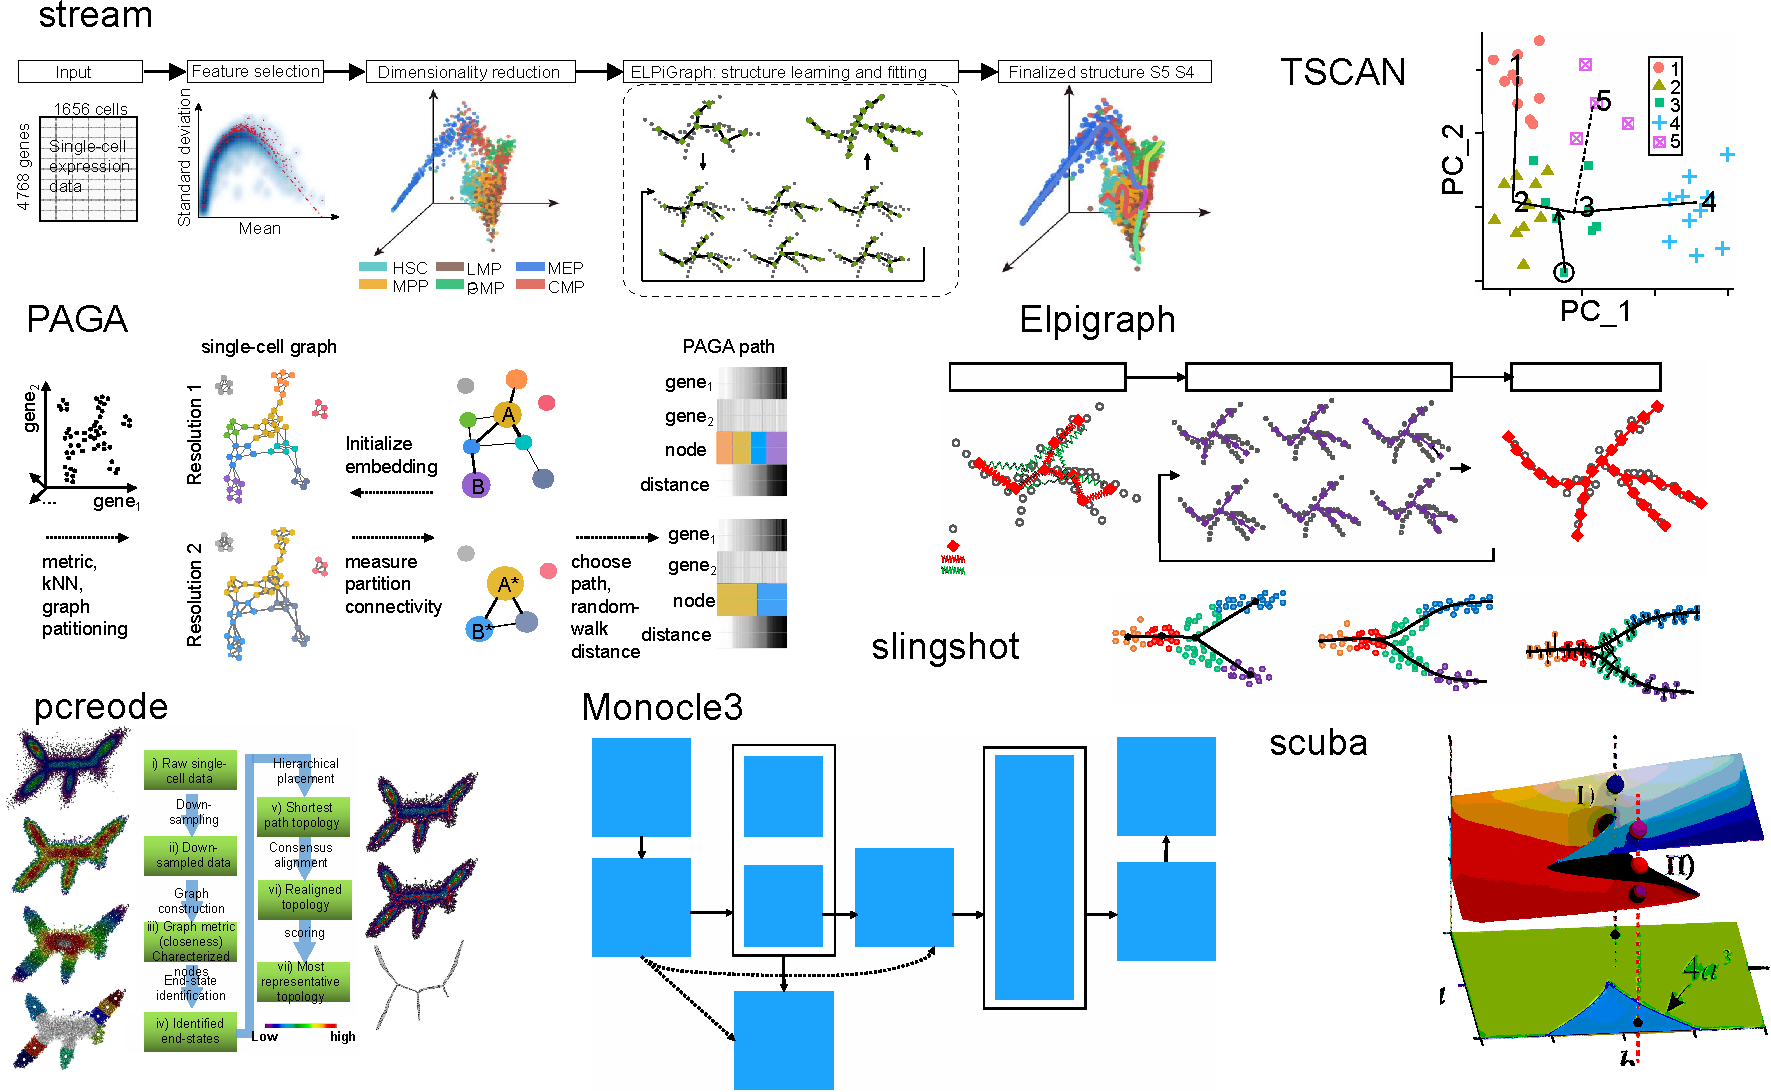
\includegraphics[width=0.95\textwidth]{TI_schemtaic/fig}
	\vspace{0.1cm}
	\caption[TI\_schemtaic.]{
	TI\_schemtaic}
	\label{fig:TI_schemtaic}
\end{figure}

\begin{table}[!ht]
	\small
	\centering
	\begin{tabular}{llllll}
		\toprule
		Name & algorithm & protocol & \#modalities  & efficiency & Reference \\
		\midrule
		MOFA     &   Matrix Decomposition &  universal &  any & slow &   \cite{argelaguet2020mofa+} \\
		Schema & Metrics learning   & universal  &  any & fast & \cite{singh2021schema} \\
		Seurat WNN	 &  WNN &  universal &  any & fast  & \cite{hao2021integrated} \\
		DIABLO &  PLS-DA & universal &  any & slow & \cite{singh2019diablo}\\
		scAI & Matrix Decomposition  &  scRNA,scATAC & 2 & slow & \cite{jin2020scai}\\
		Liger & NMF                &  shared-features&  2 & fast& \cite{kriebel2021nonnegative} \\
		Symphony\_int& CCA  &  universal & 2 & fast & \cite{kang2021symphony}\\
		\bottomrule
	\end{tabular}
	\vspace{0.1cm}
	\caption[Overview of computational integration methods]{Overview of computational integration methods.}
	\label{tab:methods_integration_overview}
\end{table}


\subsubsection{STREAM}
The Elastic principal graph:
\begin{equation}
	\begin{aligned}
& U^{phi}(X, G) = \frac{1}{|x|}\sum_{j=1}^{|V|} \sum_{i:P(i)=j} \min \left(\left\|X_i - \phi(V_j)^2, R_0^2\right\|\right) \\
&\quad + \sum_{E^{(i)}}[\lambda + \alpha (\max(2, \deg(E^{(i)}(0))) - 2)](\phi(E^{(i)}(0)) - \phi(E^{(i)}(1)))^2 \\
&\quad + \mu \sum_{S^{(j)}} \left(\phi(S^{(j)(0)}) - \frac{1}{\deg (S^{(j)(0)})} \sum_{i = 1}^{\deg (S^{(j)(0)})}\right)^2
	\end{aligned}
\end{equation}	
where $X=\{X_i\}, i = 1\cdots|X|$ is a set of points, $E^{(i)}(0)$ and $E^{(i)(1)}$ denotes the two vertices of a graph edge $E^{(i)}$, and $S^{(j)(0)},\cdots S^{(j)}(k)$ denote the vertices of the a star $S^{(j)}$ in the graph. $P(i)$ is a data point partitioning function associating each data point $X_i$ to the closest vertex index that $P(i) = \arg\min_{j=1\cdots |V|}$. $phi{V_j}$ is the mapping function that $\phi: V \rightarrow R^{m}$, which defines a position of $j$th graph vertex in the multidimensional space of data. Finally, $R_0$ is the trimming radius such that points further than $R_0$ from any nodes don't contribute to the optimization of the graph, and $\lambda$ is the edge stretching elasticity modulo regularizing the total length of the graph, and $\alpha$ is a coefficient to control the complexity of the graph. $\mu$ is the star bending elasticity that controls the smoothness of the graph.
\subsubsection{PAGA}
\subsubsection{Monocle3}
Step 1: Normalizing and pre-processing the data

To analyze a single-cell dataset, Monocle first normalizes expression values to account for technical variation in RNA recovery and sequencing depth.
Step 2: Reducing the dimensionality of the data

Next, to eliminate noise and make downstream computations more tractable, it projects each cell onto the top 50 (by default) principal components. Then, you as the user choose whether to reduce the dimensionality further using one of two non-linear methods for dimensionality reduction: t-SNE or UMAP. The former is an extremely popular and widely accepted technique for visualizing single-cell RNA-seq data. The latter is faster, and often better preserves the global structure of the data but is also newer and therefore less well tested by the single-cell community. Then, Monocle 3 will cluster your cells, organize them into trajectories, or both.
Step 3: Clustering and partitioning the cells

Monocle 3 can learn multiple disconnected or "disjoint" trajectories. This is important because many experiments will capture a community of cells that are responding to a stimulus or undergoing differentiation, with each type of cell responding differently. Because Monocle 2 assumes that all of your data is part of a single trajectory, in order to construct individual trajectories you would have to manually split up each group of related cell types and stages into different sets, and then run the trajectory analysis separately on each group of cells. In contrast, Monocle 3 can detect that some cells are part of a different process than others in the dataset, and can therefore build multiple trajectories in parallel from a single dataset. Monocle 3 achieves this by "partitioning" the cells into "supergroups" using a method derived from "approximate graph abstraction" (AGA) (Wolf et al, 2017). Cells from different supergroups cannot be part of the same trajectory.
Step 4: Learning the principal graph

Monocle 3 provides three different ways to organize cells into trajectories, all of which are based on the concept of "reversed graph embedding". DDRTree is the method used in Monocle 2 to learn tree-like trajectories, and has received some important updates in Monocle 3. In particular, these updates have massively improved the throughout of DDRTree, which can now process millions of cells in minutes. SimplePPT works similarly to DDRTree in that it learns a tree-like trajectory, but it does not attempt to further reduce the dimensionality of the data. L1Graph is an advanced optimization method that can learn trajectories that have loops in them (that is, trajectories that aren't trees).

Once Monocle 3 has learned a principal graph that fits within the data, each cell is projected onto the graph. Then, the user selects one or more positions on the graph that define the starting points of the trajetory. Monocle measures the distance from these start points to each cell, traveling along the graph as it does so. A cell's pseudotime is simply the distance from each cell to the closest starting point on the graph.
Step 5: Differential expression analysis and visualization

Once this is complete, you can run tests for genes that are specific to each cluster, find genes that vary over the course of a trajectory, and plot your data in many different ways. Monocle 3 provides a suite of regression tests to find genes that differ between clusters and over trajectories. Monocle 3 also introduces a new test that uses the principal graph directly and can help find genes that vary in complex ways over a trajectory with loops and more intricate structures.


\subsubsection{Slingshot}
\subsubsection{TSCAN}
\subsubsection{Slicer}
\subsubsection{...}
% table of single cell trajectory inference methods

% a figure of single cell trajectory inference methods theory 
\section{Discussion}
